\documentclass{article}
\usepackage{amsmath}
\usepackage{gvv-book}
\usepackage{gvv}
\usepackage{float}
\begin{document}
\begin{enumerate}
	\item Let $E$ be an event of a sample space $S$ of an experiment, then $P(S|E)=$
		\begin{enumerate}
			\item $P(S \cap E)$
			\item $P(E)$
			\item $1$
			\item $0$
		\end{enumerate}
	\item A pair of dice is thrown simultaneously. If $X$ denotes the absolute difference of the numbers appearing on top of the dice, then find the probability distribution of $X$.
	\item Airplanes are by far the safest mode of transportation when the number of transported passengers are measured against personal injuries and fatality tools.
		\begin{figure}[h]
			\centering
			     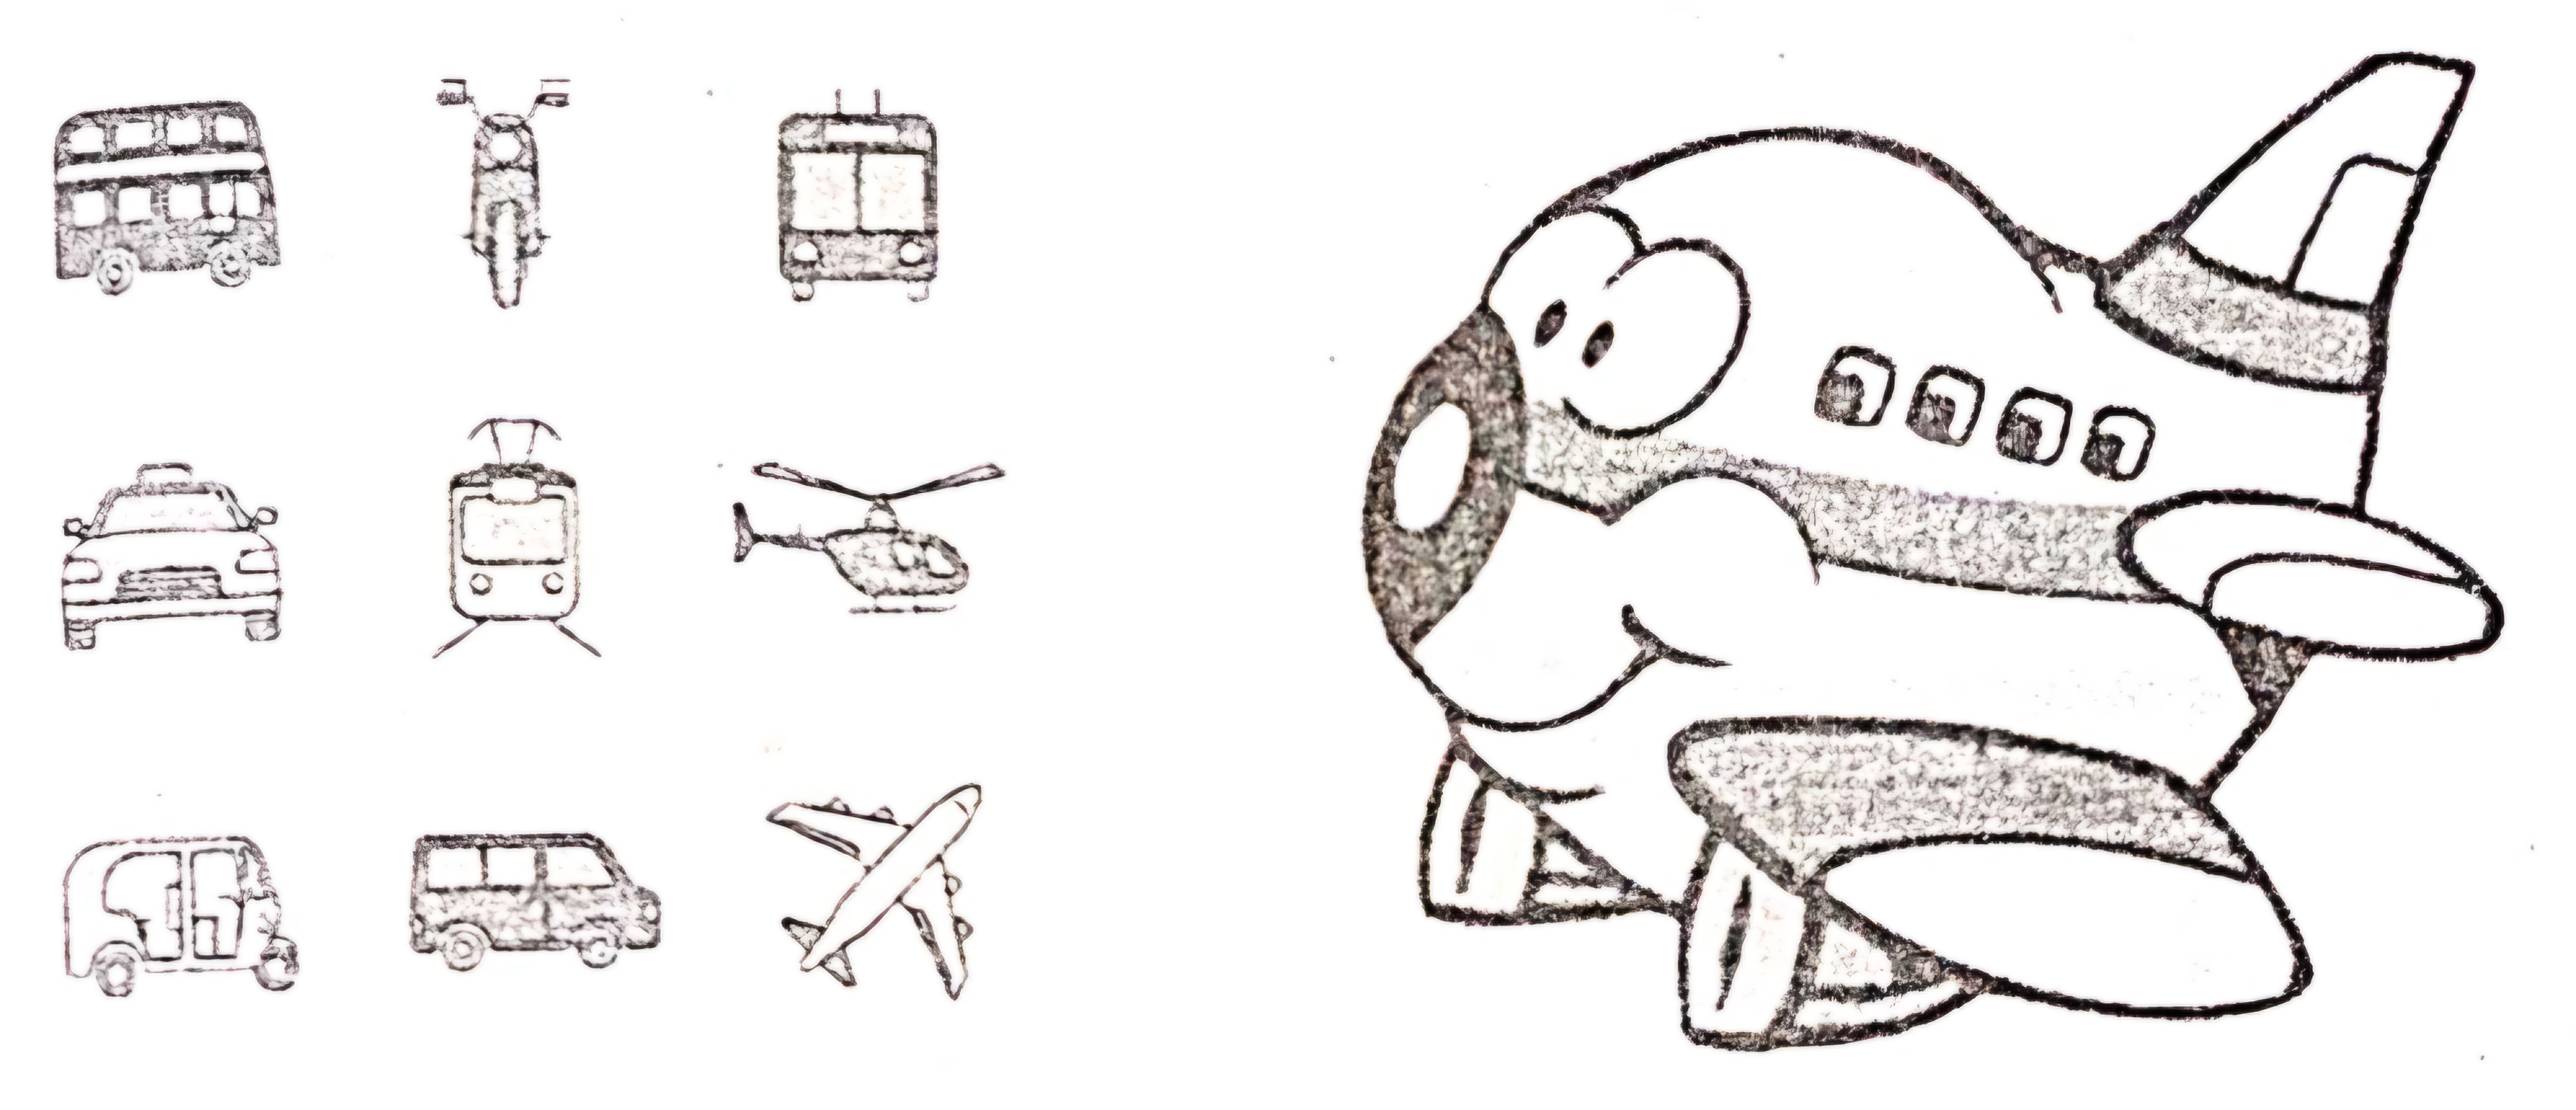
\includegraphics[width=\columnwidth]{./Figuress/Air.jpg}
			     \caption{1}
			\label{Figure}
		\end{figure}
	      Previous records state that the probability of an airplane crash is $0.00001\%$. Further, there are $95\%$ chances that there will be survivors after a plane crash. Assume that in case of no crash, all travellers survive.\\
		Let $E_{1}$ be the event that there is a plane crash and $E_{2}$ be the event that there is no crash. Let $A$ be the event that passengers survive after the journey.\\
	      On the basis of the above information, answer the following questions:
		\begin{enumerate}[label=(\roman*)]
			\item Find the probability that the airplane will not crash.
			\item Find $P(A|E_{1}) + P(A|E_{2})$.
			\item Find $P(A)$
			\item Find $P(E_{2} | A)$.
		\end{enumerate}
\end{enumerate}
\end{document}
